%!TEX root = Tesi.tex

\section{Introduzione}
Il Bluetooth è una tecnologia di comunicazione a corto raggio che esiste ormai da parecchi anni sul mercato, ma con l'avvento della specifica Low Energy, introdotta nel 2010 nella versione 4.0 e caratterizzata da un notevole risparmio in termini energetici, è stata adottata da una gran quantità di dispositivi, anche destinati a usi differenti. Basti pensare a tutti quei dispositivi che si definiscono \lq Smart\rq, dalle Televisioni agli Smartphone, dai PC agli orologi, la tecnologia ha un grande impatto sulla nostra vita di tutti i giorni.
Questa rivoluzione comunicativa prende il nome di IoT\footnote{Internet of Things, ovvero l'internet delle cose.}, il mondo dei dispositivi fisici, dove anche il più piccolo di essi, con capacità di calcolo limitate, è in grado di comunicare la propria presenza ed ottenere informazioni sulla rete proprio grazie a queste nuove tecnologie.

\'E quindi corretto chiedersi: queste tecnologie sono sicure? I danni che un malintenzionato sarebbe capace di provocare se riuscisse a manipolare a piacimento il comportamento di questi dispositivi, sono innumerevoli;
Basti pensare ad una serratura intelligente che sblocca la porta di casa quando il proprietario si trova di fronte ad essa, e se non fosse il proprietario quello davanti alla porta, ma tramite un dispositivo di ritrasmissione si spacciasse per esso? Lo stesso discorso si può applicare alle serrature ed al sistema di avvio delle recenti automobili dotate di sistema Keyless\footnote{Senza chiavi, permette l'apertura e l'avvio dell'automobile semplicemente tenendo in tasca le chiavi.}.
Restando in campo informatico, sempre più aziende stanno adottando soluzioni Smart per accedere ai PC, senza dover inserire manualmente la classica password; Apple da la possibilità ai propri utenti di sbloccare il  MacBook tramite il loro Apple Watch, semplicemente avvicinandolo allo schermo; un malintenzionato riuscirebbe con facilità a rubare i dati personali di un utente se riuscisse a sfruttare una falla di questo meccanismo di sblocco.

\'E proprio su questi presupposti che si basa questo progetto di tesi, testare la sicurezza del protocollo Bluetooth tramite la creazione di uno Sniffer a basso costo che permetta di visualizzare ed analizzare i pacchetti scambiati da due dispositivi durante tutta la durata di una connessione. L'implementazione di uno Sniffer è utile anche per un'attività di Debug nello sviluppo delle applicazioni; permette di vedere realmente la composizione del pacchetto inviato e quindi di trovare facilmente errori nell'applicativo.
Uno degli sviluppi futuri è quello riuscire a creare un ripetitore di segnale tra due punti, basandosi sul lavoro svolto in questa tesi, che faccia credere ai dispositivi di essere a stretto contatto quando in realtà li separa una distanza maggiore; questo dimostrerebbe che un dispositivo Bluetooth Low Energy è vulnerabile ad attacchi di tipo Relay, e forzerebbe i costruttori a risolvere queste vulnerabilità e quindi a migliorare la sicurezza del protocollo.

\newpage 

\subsection{Alternative}
Sul mercato esistono già prodotti di sniffing completi, funzionanti e pronti per essere usati; il problema di questi dispositivi è che sono costosi e per la maggior parte non Open Source. La principale limitazione di ciò è che il codice su cui si basano non può essere manipolato a piacimento secondo le proprie esigenze e quindi questi programmi possono essere unicamente usati per lo scopo per cui sono stati creati. Se uno sviluppatore in possesso di uno di questi dispositivi a Closed Source volesse cambiare un leggero aspetto di un programma di Sniffing preconfezionato dovrebbe riscriversi completamente il codice da zero, con un enorme dispendio di tempo e risorse per simulare il comportamento di un applicativo già esistente.

\subsection*{Ubertooth One}
Ubertooth One è un progetto Open Source di sviluppo su reti Wireless, capace di comunicare utilizzando il protocollo trasmissivo BLE. Sulla loro pagina GitHub \cite{ubertooth_github_web} è possibile reperire, oltre ai vari progetti sviluppati appositamente, anche il disegno delle componentistiche Hardware, per poter assemblarlo e costruirlo privatamente o addirittura modificarlo secondo le proprie necessità.

\begin{figure}[H]
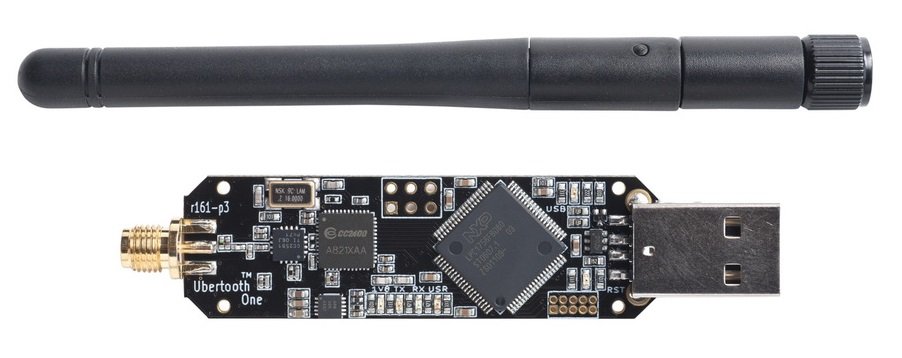
\includegraphics[width=340pt]{ubertooth_one}
\centering
\caption{UberTooth One}
\end{figure}

Si hanno ha disposizione vari progetti creati per questo dispositivo, tra i tanti va citato \lq Bluetooth Captures in PCAP\rq  \cite{ubertooth_pcap_web} che permette di ascoltate, in una sorta di modalità promiscua, tutte le comunicazioni bluetooth su un certo canale, oppure tramite l'ascolto di una CONNECT\_ REQ. seguire una connessione. Permette ulteriormente di interfacciarsi con l'applicazione \emph{WIRESHARK}\footnote{\'E un software per analisi di protocolli o pacchetti utilizzato per la soluzione di problemi di rete, per l'analisi e lo sviluppo di protocolli o di software di comunicazione.} per visualizzare in tempo reale il traffico BLE, applicare filtri su indirizzi o potenza del segnale ed inviare pacchetti personalizzati.

L'aspetto negativo di questa soluzione sta nel costo, difatti ad oggi si trova in commercio ad un prezzo che si aggira attorno ai 150\euro  + spese di consegna \cite{ubertooth_reseller_web}.

\subsection*{Bluefruit LE sniffer}
Il Bluefruit LE monta al suo interno il chip della Nordic nRF51822 che viene venduto già programmato con un software che trasforma il dispositivo in uno sniffer di traffico Bluetooth Low Energy. I pacchetti raccolti vengono mandati in automatico a Wireshark  dove possono essere visualizzati con un'opportuna struttura che facilita la comprensione delle varie parti del pacchetto, senza far riferimento al manuale Bluetooth Core.

\begin{figure}[H]
\includegraphics[width=320pt]{bluefruit_sniffer}
\centering
\caption{Bluefruit LE Sniffer - Bluetooth Low Energy (BLE 4.0) - nRF51822}
\end{figure}

Le limitazioni di questa soluzione sono molteplici; il software che viene installato per gestire il dispositivo come sniffer non è open source; il tool che permette l'interfacciamento tra il dispositivo e wireshark esiste solo per l'ambiente windows. Il dispositivo così come è venduto non può essere programmato, necessita infatti di un programmatore esterno, come il J-Link venduto ad un costo che si aggira sui 15\euro .
Il costo del dispositivo è di circa 25\euro\ paragonabile al prezzo di acquisto di un RedBear Nano2.

\newpage 

\subsection*{nRF52 DK}\label{nordic_board}
La board di sviluppo nRF52 DK della Nordic Semiconductor è una periferica di sviluppo versatile e completa per testare applicazioni BLE, ANT e protocolli proprietari che usano le frequenze 2.4GHz. Integra 4 led e 4 bottoni che possono essere usati rispettivamente per ricevere informazioni sullo stato di funzionamento del dispositivo e per impartire comandi a quest'ultimo.

\begin{figure}[H]
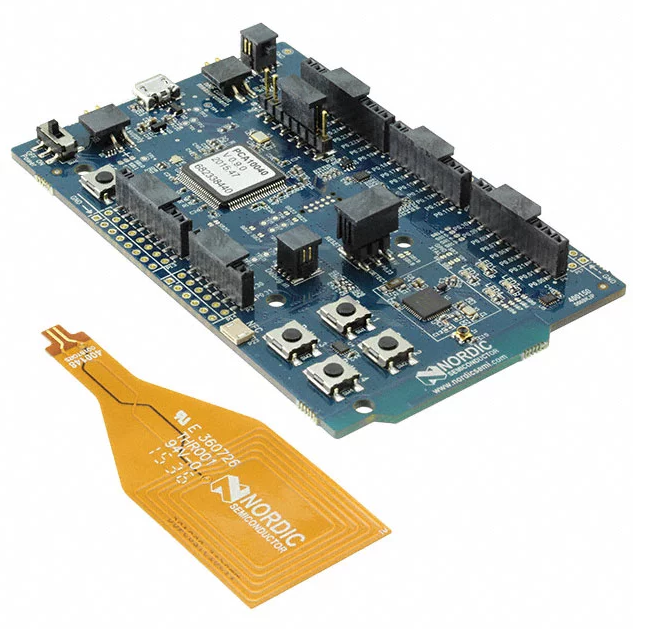
\includegraphics[width=320pt]{nrf52_dk}
\centering
\caption{Board di sviluppo NRF52\_ DK creata dalla società Nordic Semiconductor.}
\end{figure}

Essendo ufficialmente supportata dalla stessa Nordic, lo sviluppatore ha a disposizione molti tool per lo sviluppo e il testing di applicazioni. Esiste anche un software di sniffing preconfezionato che permette di svolgere tutte le operazioni di sniffing direttamente da wireshark, tra cui la possibilità di seguire in maniera del tutto automatizzata una connessione e vedere in tempo reale la composizione e il significato di tutti i pacchetti scambiati. 
Sfortunatamente questo software esiste solo per windows e non è open source, quindi non è utilizzabile per lo scopo di questa tesi.
Oltretutto il costo di questa board di sviluppo è di circa 40\euro\ più spese di consegna, più alto di quello di un Nano2.

\subsection*{USRP EttusB210}
Il B210 fornisce una singola scheda integrata su una piattaforma USRP\footnote{Universal Software Radio Peripheral, componente della Ettus Research di tipo Software-defined radio (SDR)} con una copertura continua di frequenza da 70 Mhz a 6 GHz. Progettato per la sperimentazione a basso costo, combina il ricetrasmettitore di conversione diretta RFC AD9361 che fornisce fino a 56 MHz di larghezza di banda in tempo reale, un FPGA\footnote{Field Programmable Gate Array, circuito integrato le cui funzionalità sono programmabili via software}, Spartan6 XC6SLX150 open-source e riprogrammabile, ed una connettività ad alta velocità utilizzando USB 3.0 con canale di alimentazione dedicato. Il B210 consente un facile e veloce sviluppo con il toolkit di sviluppo software GNURadio, consentendo così di sperimentare con un'ampia gamma di segnali e bande di frequenza, inclusi trasmissioni FM, TV, cellulari, Wi-fi e Bluetooth.

\begin{figure}[H]
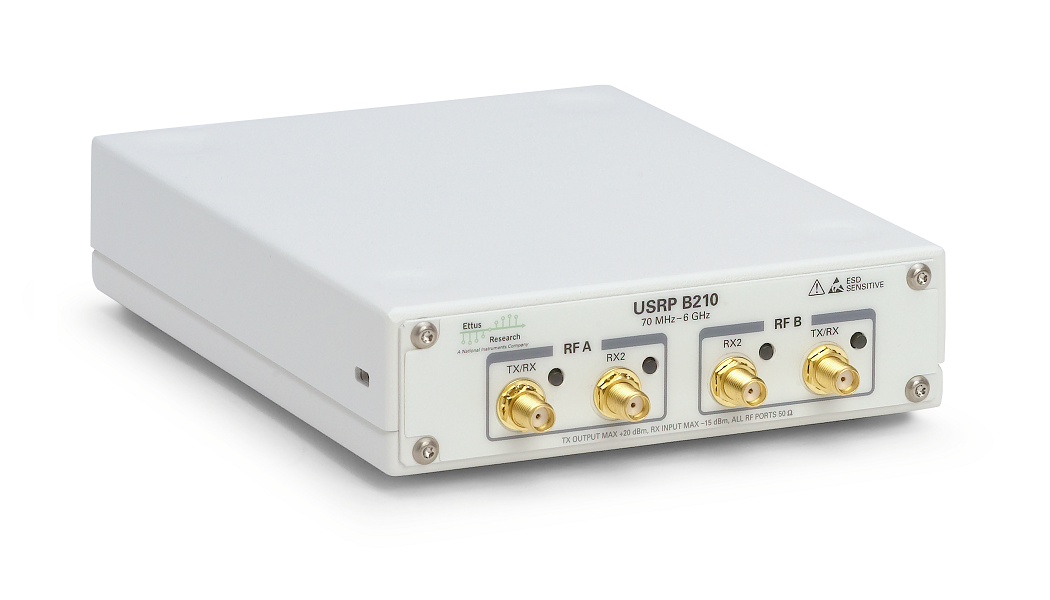
\includegraphics[width=340pt]{usrp_b210}
\centering
\caption{USRP Ettus B210, Ettus Research una società della compagnia National Instrument. }
\end{figure}

La massima banda trasmissiva campionabile in tempo reale con questo dispositivo è di 56 MHz a 61,44 MS/s\footnote{Mega Sample al secondo, unità di misura della frequenza di campionamento.} inferiore alla banda trasmissiva del Bluetooth Low Energy. Il costo di questa board è molto elevato rispetto alle precedenti soluzioni, essendo di circa 1.250\euro\ .
Per questo progetto disponiamo comunque di due di questi dispositivi, essendo stati acquistati dall'università in precedenza, che riescono a coprire gli 80 MHz di banda trasmissiva BLE. Si sono rilevati molto utili per capire ciò che realmente passa nell'etere a quelle frequenze. Il dispositivo campiona qualsiasi segnale nella banda trasmissiva, creando una gran quantità di dati che devono essere poi analizzati e filtrati con un software creato appositamente per estrarne i pacchetti BLE di nostro interesse.

\subsection*{Frontline BPA Low Energy}
Progettato e commercializzato dalla società TELEDYNE LECROY, il Frontline BPA Low Energy Bluetooth protocol analyzer è un dispositivo creato appositamente per la funzione di sniffing di pacchetti BLE. Utilizzabile unicamente su sistemi Windows, viene venduto con un applicativo, non open source, da installare che permette di visualizzare tutto il traffico Bluetooth LE in tempo reale, salvare tutto ciò che è stato catturato ed analizzarlo nel dettaglio; con opportuni filtri risulta molto facile trovare il pacchetto di interesse tra gli svariati catturati e vederne nel dettaglio tutte le componenti con i loro valori. \'E interfacciabile anche con WireShark, permettendo quindi all'utente di usufruire delle potenzialità della piattaforma ed integrarlo in progetti già esistenti.

\begin{figure}[H]
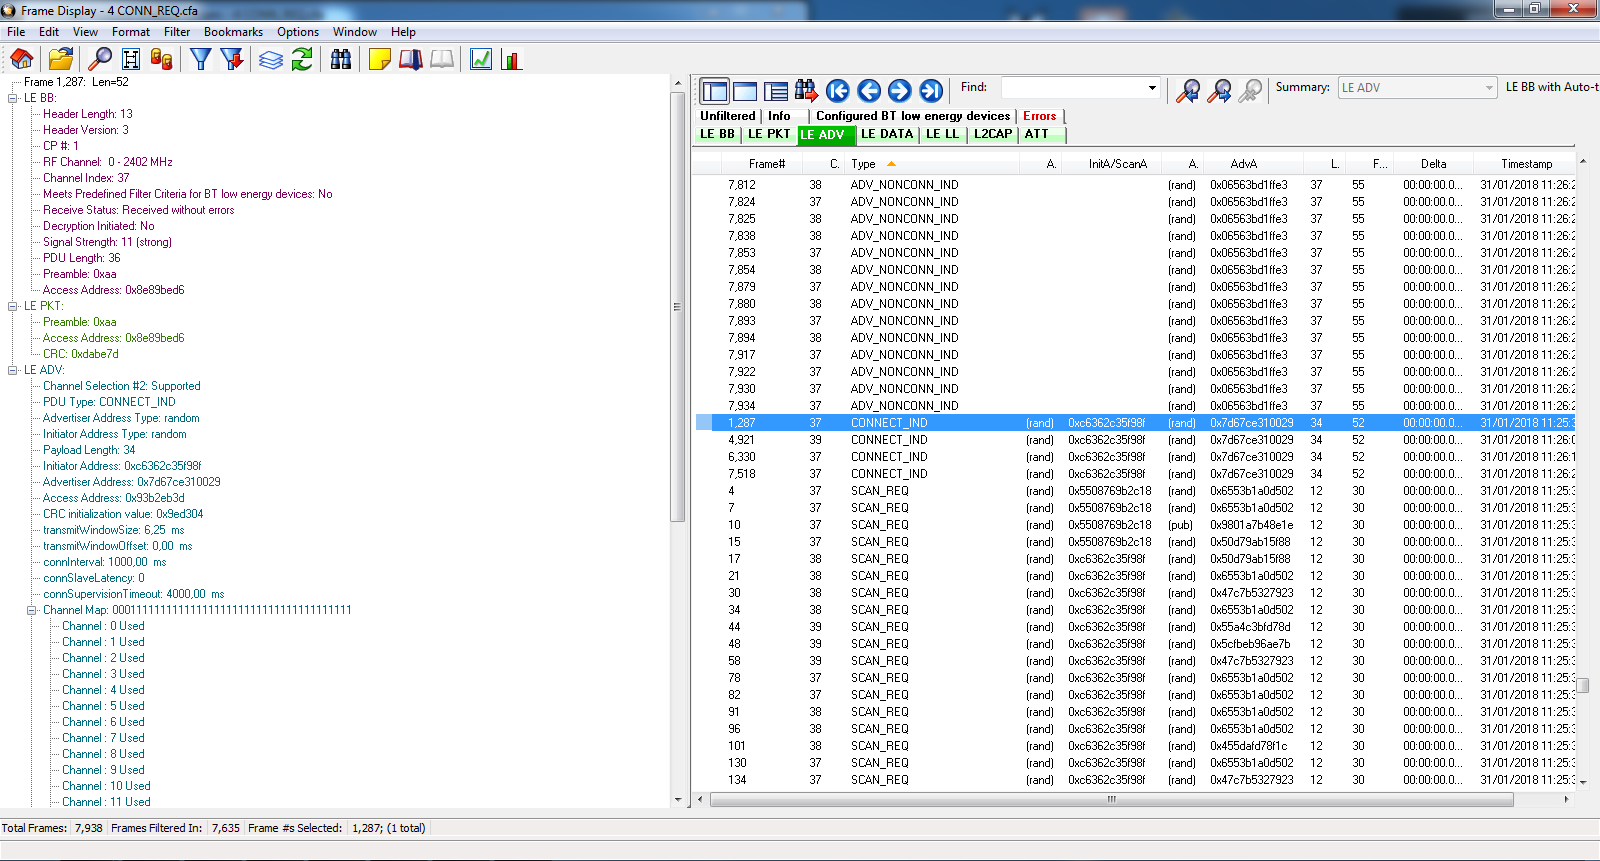
\includegraphics[width=340pt]{frontline_sw}
\centering
\caption{Schermata del software di analisi del traffico ble, distribuito con il dispositivo BPA di sniffing. }
\end{figure}

\'E stato utilizzato come supporto per lo sviluppo del progetto di tesi, in quanto è stato possibile averne uno a disposizione; si è rivelato utile per conoscere esattamente il valore dei vari campi, sopratutto di quelli composti da pochi bit, che il dispositivo nano2 tendeva ad inviare secondo un ordine che non era quello delle specifiche BLE. Conoscendo esattamente il nome del campo ed il relativo valore, fornito dal software di analisi utilizzato con lo sniffer BPA, è stato quindi possibile risalire all'esatta posizione dello stesso all'interno di ciò che veniva catturato dal dispositivo della RedBear, riuscendo a mappare l'esatta disposizione di tutti i campi del pacchetto. Sfortunatamente i documenti che mette a disposizione la società che ha creato il Nano2 sono scarsamente dettagliati e privi di molte informazioni essenziali, si è perciò reso necessario appoggiarsi su strumenti più professionali per capire come funzionasse esattamente e quindi per poter procedere con lo sviluppo di uno Sniffer a basso costo.
Il dispositivo è disponibile sul mercato ad un costo decisamente elevato, che si aggira attorno ai 900\euro\ .